\documentclass{../zkdl-presentation-template}

\title[Криптографія]{\textbf{Практичне №7.Криптосистеми Ель-Гамаля. RSA. Добування коренів квадратних за модулем}}

\date{4.11.2025}


\begin{document}
    \frame{
        \titlepage
    }
  
    \begin{frame}{Plan}
        \tableofcontents
    \end{frame}

\section{Криптосистема Ель-Гамаля} % Note all sections and subsections are automatically placed in your table of contents

%------------------------------------------------
\begin{frame}
    \frametitle{Протокол}
    \texttt{Генерування ключів.} Аліса обирає $p$ -- просте число та елемент $g$ великого простого порядку $q$ за модулем $p$ (зокрема $g\in \mathbb{Z}^*_p$ може бути і генератором). Також Аліса обирає випадкове значення $x\in_R\mathbb{Z}_q$ та обчислює число $y:=g^x\text{ mod }p$. Число $x$ є секретним ключем Аліси, а трійка $(y,p,g)$ - відкритим ключем Аліси.
    
\texttt{Шифрування.} Боб бажає зашифрувати для Аліси повідомлення $g\in \mathbb{Z}^*_p$. Для цього Боб генерує одноразовий секретний ключ $k\in_R\mathbb{Z}_q$ та обчислює значення:
 \begin{gather*}
     c_1=g^k(\text{ mod }p)\\
     c_2=m\cdot y^k (\text{ mod }p)
 \end{gather*}
Пара чисел $c=(c_1,c_2)$ є шифротекстом повідомлення $m$.
\texttt{Розшифрування.} Одержавши шифротекст $c=(c_1,c_2)$, Аліса обчислює значення $m$: $m:=c_2\cdot (c_1)^{-x}\text{ mod }p$ .

\end{frame}

%------------------------------------------------
\begin{frame}
    \frametitle{Задачі}
        \begin{block}{}
        Покажіть, що процедура розшифрування схеми Ель-Гамаля дійсно повертає правильне значення відкритого тексту.
         \begin{gather*}
     c_1=g^k(\text{ mod }p)\\
     c_2=m\cdot y^k (\text{ mod }p)
 \end{gather*}
 $m:=c_2\cdot (c_1)^{-x}\text{ mod }p$ .
    	\end{block}
        \begin{figure}
            \centering
            
\includegraphics[width=1\linewidth]{2-crypto-sym/images/cells_small.png}
            \label{fig:placeholder}
        \end{figure}
    
\end{frame}
%------------------------------------------------
\begin{frame}
    \frametitle{Задачі}
        \begin{block}{}
        Зламайте схему Ель-Гамаля, якщо $k=\frac{q}{2}$
                    \centering
            
\includegraphics[width=1\linewidth]{2-crypto-sym/images/cells.png}

    	\end{block}
    
\end{frame}
%------------------------------------------------
\begin{frame}
    \frametitle{Схема Горнера}
    \centering
            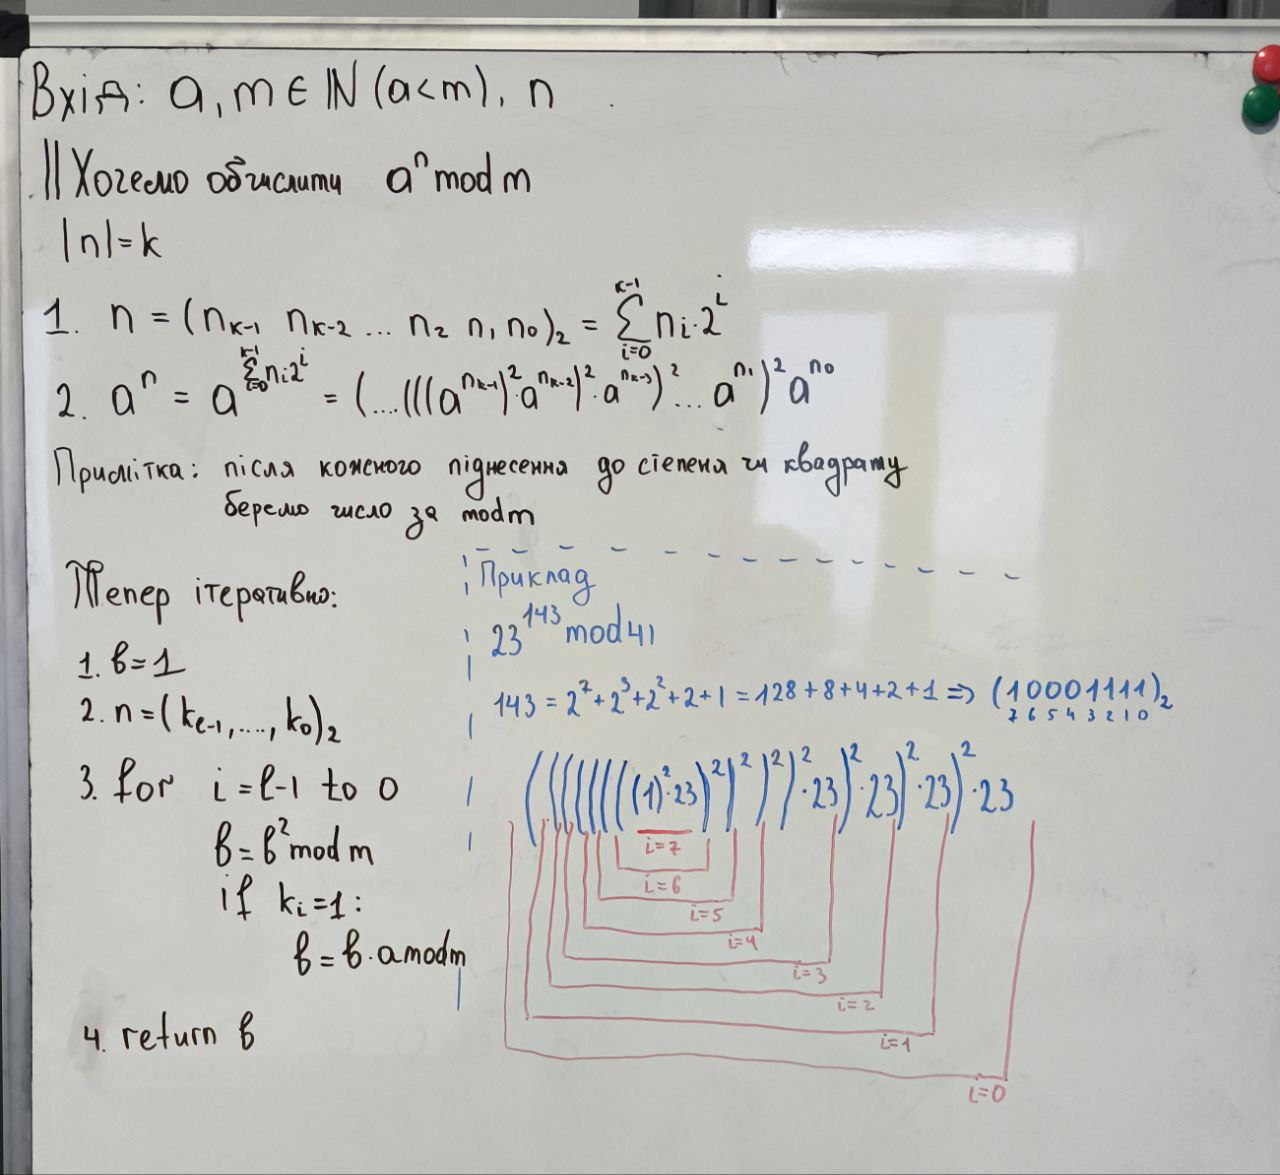
\includegraphics[width=0.8\linewidth]{7-crypto-practice/gorner.jpg}
    
\end{frame}
%------------------------------------------------
\begin{frame}
    \frametitle{Задачі}
        \begin{block}{}
        Задано параметри $p=29,g=2,m=9,k=5$, секретний ключ підписувача повідомлення $x=4$. Визначити відкритий ключ перевіряючого повідомлення. Сформувати та перевірити ЦП. 
                    \centering
            
\includegraphics[width=1\linewidth]{2-crypto-sym/images/cells.png}

    	\end{block}
    
\end{frame}
%------------------------------------------------
\section{Протокол RSA}
%------------------------------------------------
\begin{frame}
    \frametitle{Задачі}
        \begin{block}{}
        1. Переформулюйте криптосистему RSA для випадку простого модуля.
        \begin{enumerate}
            \item[a)] покажіть. що така система не є стійкою;
            \item[b)]  покажіть, що якщо обрати $p=q$, то опис криптосистеми стане некоректним, а система стане нестійкою.
        \end{enumerate}

        2. Покажіть, як за відомим $n$ та значенням функції Ойлера для $\phi(n)$ обчислити значення  $p$ та $q$
            
\includegraphics[width=1\linewidth]{2-crypto-sym/images/cells_small.png}

    	\end{block}
    
\end{frame}
%------------------------------------------------
\begin{frame}
    \frametitle{Задачі}
        \begin{block}{}
        Доведіть, що процедура розшифрування RSA коректно розшифровує відкритий текст $m$ навіть якщо $\mathsf{GCD}(m,n)>1$. Оцініть ймовірність того, що випадково обране повідомлення буде невзаємнопростим із модулем $n$.
            
\includegraphics[width=0.95\linewidth]{2-crypto-sym/images/cells.png}
    	\end{block}
\end{frame}
%------------------------------------------------
\section{Корені квадратні за модулем}
%------------------------------------------------
\begin{frame}
    \frametitle{Добування квадратних коренів за простим модулем}
    Можемо виділити три випадки представлення $x^2\equiv a\text{ mod }p$:

    \begin{align*}
        p=4k+3 \qquad& \qquad p=8k+5 \\ \\
        p=&8k+1
    \end{align*}
\begin{block}{}
     Для кожного випадку, ми маємо ОБОВ'ЯЗКОВО перевірити чи є число $a$ квадратичним лишком. Якщо ні, то ми не зможемо обрахувати значення кореня. Перевірка відбувається за символом Лежандра:
    \begin{align*}
        \left(\frac{a}{p}\right)\overset{?}{=}1
    \end{align*}
\end{block}
   
\end{frame}
%------------------------------------------------
\begin{frame}
    \frametitle{ $x^2\equiv a\text{ mod }4k+3$}
    Є найпростішим випадком у добуванні кореня квадратного за модулем. Неважко помітити:
    \begin{gather*}
        a^{(p-1)/2}= a^{2k+1} = 1 \text{ mod } p \quad\Rightarrow\quad  a^{2k+2} = a \text{ mod } p  \quad\Rightarrow
        \\
        \\
        \mathbf{x = \pm a^{k+1} \text{ mod } p}
    \end{gather*}
\end{frame}
%------------------------------------------------
\begin{frame}
    \frametitle{$x^2\equiv a\text{ mod }8k+5$:}
    \begin{figure}
        \centering
        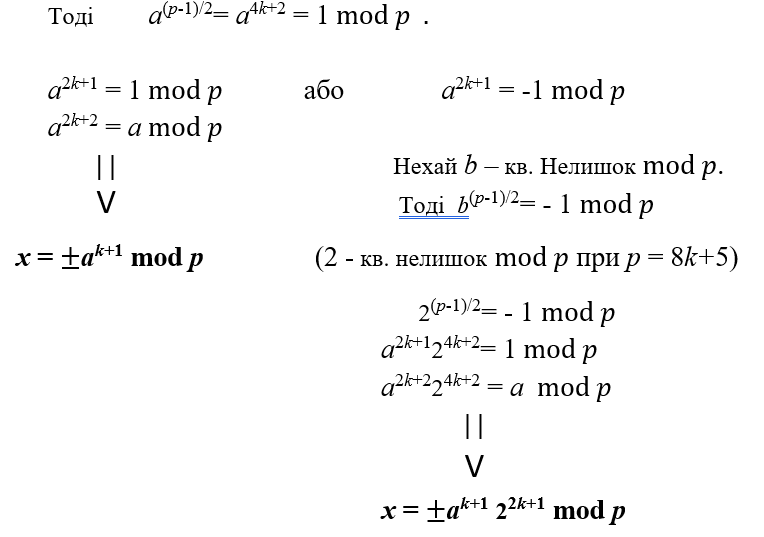
\includegraphics[width=0.9\linewidth]{7-crypto-practice/11.png}
        \label{fig:placeholder}
    \end{figure}
\end{frame}
%------------------------------------------------
\begin{frame}
    \frametitle{$x^2\equiv a\text{ mod }8k+1$:}
    \begin{figure}
        \centering
        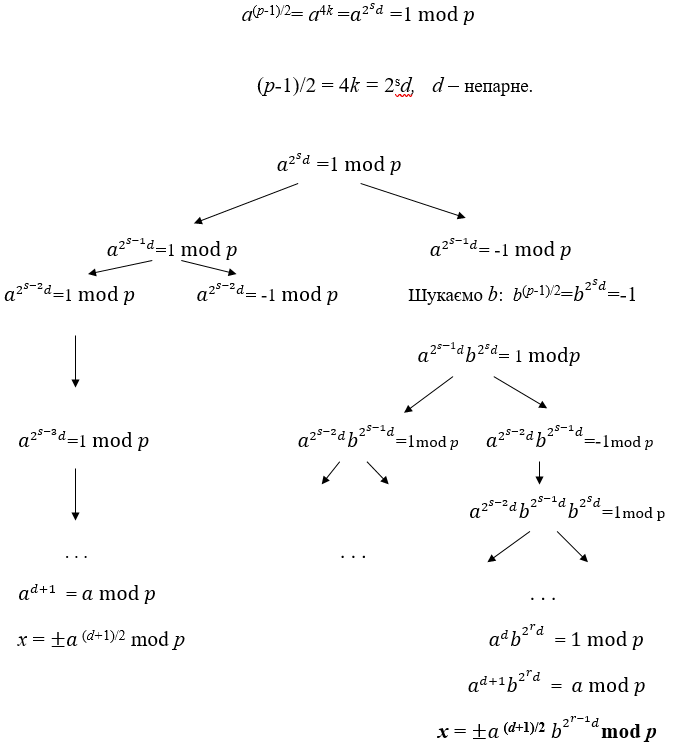
\includegraphics[width=0.65\linewidth]{7-crypto-practice/12.png}
        \label{fig:placeholder}
    \end{figure}
\end{frame}
%------------------------------------------------
\begin{frame}
    \frametitle{Універсальний метод :)}
    \begin{figure}
        \centering
        
\includegraphics[width=1\linewidth]{2-crypto-sym/images/cells.png}
        \label{fig:placeholder}
    \end{figure}
    
\end{frame}
%------------------------------------------------
\begin{frame}
    \frametitle{Добування за складеним модулем $n=pq$}
    Очевидно, що для добування кореня квадратного від числа $a$ за складеним модулем $n=pq$, число повинно бути квадратичним лишком як за $q$, так і за $q$. Якщо ці умови виконуються, то ми можемо обчислити наступні рівняння:
    \begin{gather*}
        x^2=a\text{ mod }p \qquad\qquad x^2=a\text{ mod }q
    \end{gather*}
    Кожне рівняння дає по два відповідні корені $\pm x_p, \pm x_q$. Тоді розв'язок початкового рівняння буде задовольняти наступній системі рівнянь:
    \begin{align*}
         \left\{ \begin{array}{r}
x=\pm x_p \text{ mod } p  \\ 
x=\pm x_q \text{ mod } q 
\end{array}\right.
    \end{align*}
    Розписавши цю систему як 4 системи і вирішивши кожну із них за Китайською теоремою про лишки, отримаємо \textbf{4 корені}.
    
\end{frame}
%------------------------------------------------

    \begin{frame}[plain, standout]
    \begin{figure}
        \centering
        
\includegraphics[width=0.9\linewidth]{Cryptocats.jpg}
        \label{fig:placeholder}
    \end{figure}
    \centering
    \LARGE
    \textbf{Питання?} \\

    \vspace{0.2cm} \Huge \ding{170} \large \\

  \end{frame}
\end{document}